\documentclass[twoside,11pt]{article}

\usepackage{../Style/feuille-tp}

\formation{IUT - Département Informatique}
\matiere{Théorie des langages}
\titre{Exercices sur les langages rationnels}
\sigle{Maths \\ 2013-2014}


\sloppy

\begin{document}


\maketitle

\begin{multicols}{2}
\section{Construction d'automates}

\Q Construire un automate sur l'alphabet  $\{ a, b, c \}$
pour les expressions régulières suivantes

\begin{itemize}
\item $E_1 = a {(b + b c^* c)}^* c$
\item $E_2 = {(b+c)}^* a {(a+b+c)}^*$
\item $E_3 = {(b+c)}^* { (ab {(b+c)}^* ) }^*$
\end{itemize}

\Q Déterminisez-les.



\section{Langages}

\Q Soit $w$ un mot sur un alphabet $A$. Montrez que le langage des
mots qui contiennent $w$ comme facteur est rationnel.

\Q Soit $L$ un langage rationnel. Montrez que les ensembles suivants
sont des langages rationnels :
\begin{enumerate}
\item $Pref(L)$, les préfixes des mots appartenant à $L$.
\item $Suff(L)$, les suffixes.
\item $Fact(L)$, les facteurs.
\item $Sub(L)$, les sous-mots de mots de $L$. Par définition, $u$ de
  longueur $n$, est un sous-mot de $v$ (de longueur $m$) si il existe
  une suite de $n$ entiers $0 < i_1 < i_2 < ...< i_n < m$ tels que
  $u_k = v_{i_k}$ pour tout $k$ entre 1 et $n$. 

Par exemple $aace$ est un sous-mot de $aaabbbccddee$.
\end{enumerate}
\section{Expressions régulières}

Construisez une expression régulière pour l'automate suivant :

\end{multicols}


\begin{center}
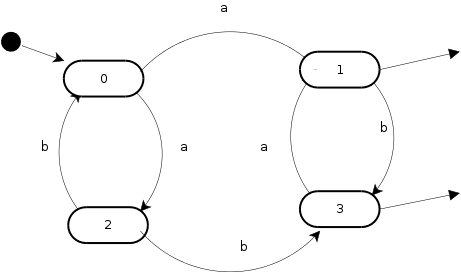
\includegraphics[width=0.8\linewidth]{../dia/exoauto}
\end{center}




\end{document}
